\section{Auswertung}
\label{sec:Auswertung}

Im folgenden wird sowohl die Strömungsgeschwindigkeit in Abhängigkeit des Prismawinkels $\varphi$ ausgewertet, als auch ein Strömungsprofil für den
mittleren Schlauch angelegt. Die ausgewerteten Messwerte werden grafisch dargestellt.

\subsection{Auswertung der Strömungsgeschwindigkeit}
\label{subsec:stroemi}
Als erstes wird zu den jeweiligen Winkeln $\varphi$, die am Prisma eingestellt wurden, der zugehörige Dopplerwinkel $\alpha$ nach Gleichung (\ref{eqn:alpha})
berechnet und in \autoref{tab:winkel} eingetragen.
\begin{table}[H]
  \centering
  \caption{Prisma- und Dopplewinkel.}
  \label{tab:winkel}
  \begin{tabular}{c c}
    \toprule
    Prismawinkel $\varphi$ & Dopplerwinkel $\alpha$ \\
    \midrule
    $\SI{15}{\degree}$ & $\SI{80,06}{\degree}$ \\
    $\SI{30}{\degree}$ & $\SI{70,53}{\degree}$ \\
    $\SI{45}{\degree}$ & $\SI{61,87}{\degree}$ \\
    \bottomrule
  \end{tabular}
\end{table}

\noindent
Es wird die Strömungsgeschwindigkeit in Abhängigkeit des Dopplerwinkels $\alpha$ untersucht. Hierzu wird ein Rohr mit einem Außendurchmesser von $\SI{20}{\milli\meter}$
und einem Innendurchmesser von $\SI{16}{\milli\meter}$ verwendet und an den drei verschiedenen Winkeln ausgewertet. Die Messwerte sind der \autoref{tab:AufgabeA} zu entnehmen.
An der Zentrifugalpumpe, die die Strömungsgeschwindigkeit regelt, wurde in einem Bereich von $3000 \,\text{rpm}$ bis $7000 \,\text{rpm}$ in Schrittweiten von $1000 \,\text{rpm}$ gemessen. Dies entsricht den in der
Tabelle verzeichneten Abweichungen von der maximalen Leistung ($8400\, \text{rpm}$). Sie sind gegenüber der Differenz der maximalen und minimalen Frequenz $\upDelta \nu = f_{\text{max}} - f_{\text{mean}}$ dargestellt.
\begin{table}[H]
  \centering
  \caption{Frequenzdifferenz $\upDelta \nu$ in Abhängigkeit der Pumpleistung.}
  \label{tab:AufgabeA}
  \begin{tabular}{c c c c c c c}
    \toprule
    Prismawinkel $\varphi$ & $35,7 \%$ & $47,62 \%$ & $59,52 \%$ & $71,43 \%$ & $83,3 \%$\\
    \midrule
    $\SI{15}{\degree}$ & $\SI{45}{\hertz}$ & $\SI{62}{\hertz}$ & $\SI{91}{\hertz}$ & $\SI{175}{\hertz}$ & $\SI{186}{\hertz}$ \\
    $\SI{30}{\degree}$ & $\SI{55}{\hertz}$ & $\SI{102}{\hertz}$ & $\SI{152}{\hertz}$ & $\SI{246}{\hertz}$ & $\SI{355}{\hertz}$ \\
    $\SI{45}{\degree}$ & $\SI{96}{\hertz}$ & $\SI{184}{\hertz}$ & $\SI{298}{\hertz}$ & $\SI{461}{\hertz}$ & $\SI{643}{\hertz}$ \\
    \bottomrule
  \end{tabular}
\end{table}

\noindent
Die Strömungsgeschwindigkeiten $v$ folgen nun, indem die \autoref{eqn:df} umgestellt wird. Die berechneten Strömungsgeschwindigkeiten sind in \autoref{tab:stroemungsgeschw} eingetragen.
\begin{table}[H]
  \centering
  \caption{Strömungsgeschwindigkeiten in Abhängigkeit der Pumpleistung.}
  \label{tab:stroemungsgeschw}
  \begin{tabular}{c c c c c c c}
    \toprule
    Prismawinkel $\varphi$ & $35,7 \%$ & $47,62 \%$ & $59,52 \%$ & $71,43 \%$ & $83,3 \%$\\
    \midrule
    $\SI{15}{\degree}$ & $\SI{855}{\meter\per\second}$ & $\SI{62}{\meter\per\second}$ & $\SI{91}{\meter\per\second}$ & $\SI{175}{\meter\per\second}$ & $\SI{186}{\meter\per\second}$ \\
    $\SI{30}{\degree}$ & $\SI{55}{\meter\per\second}$ & $\SI{102}{\meter\per\second}$ & $\SI{152}{\meter\per\second}$ & $\SI{246}{\meter\per\second}$ & $\SI{355}{\meter\per\second}$ \\
    $\SI{45}{\degree}$ & $\SI{96}{\meter\per\second}$ & $\SI{184}{\meter\per\second}$ & $\SI{298}{\meter\per\second}$ & $\SI{461}{\meter\per\second}$ & $\SI{643}{\meter\per\second}$ \\
    \bottomrule
  \end{tabular}
\end{table}

\noindent
Die Strömungsgeschwindigkeiten $v$ folgen nun, indem die Formel \eqref{eqn:df} umgestellt wird. In der folgenden \autoref{fig:plot} sind die Werte aus der 
berechneten Strömungsgeschwindigkeiten visuell gegen den Quotient aus der Frequenzdifferenz $\upDelta \nu$ und $\cos(\alpha)$ dargestellt.
\begin{figure}[H]
  \centering
  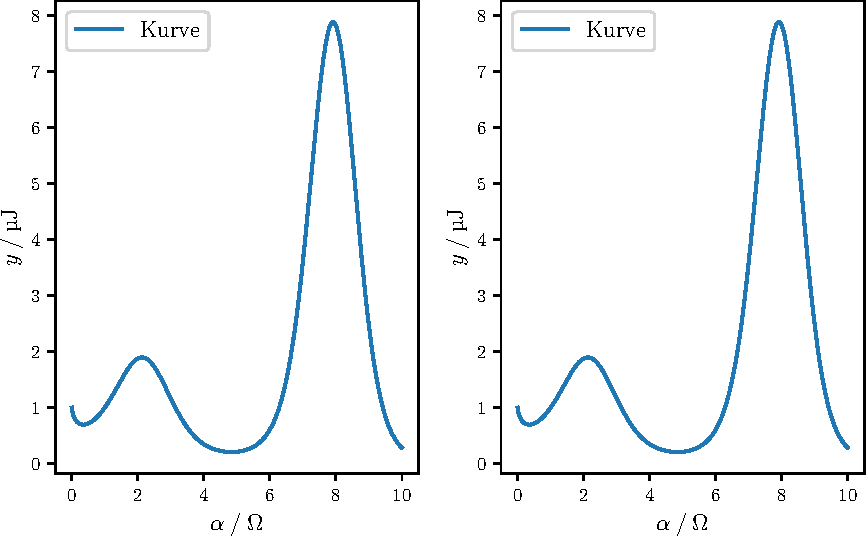
\includegraphics[width=0.75\textwidth]{build/plot.pdf}
  \caption{Messwerte für drei verschiedene Einstrahlwinkel gegen die berechnete Strömungsgeschwindigkeit $\frac{\upDelta\nu}{\cos(\alpha)}$.}
  \label{fig:plot}
\end{figure}

\subsection{Auswertung des Strömungprofils}
\label{subsec:StroemiProf}
Im zweiten Teil des Versuches wird für einen Schlauch mit einem Außendurchmesser von $\SI{15}{\milli\meter}$ und einem Innendurchmesser von $\SI{10}{\milli\metre}$ ein
Strömungsprofil unter einem Einfallwinkel von $\SI{45}{\degree}$ angelegt. Die Messwerte für eine Leistung von $70\%$ sind in \autoref{tab:Werte1} und für $45\%$ in 
\autoref{tab:Werte2} zu finden. Dargestellt sind die Messtiefe des Ultraschalls, die Signalstärke und die Fließgeschwindigkeit der Flüssigkeit.
Die Werte sind außerdem in \autoref{fig:plot2} für eine Pumpleistung von $45 \%$ und in \autoref{fig:plot3} für eine Pumpleistung von $70 \%$ eingetragen.
\begin{table}[H]
  \centering
  \caption{Messwerte des zweiten Aufgabenteils bei 45 \% Leistung (3.870 rpm) des Gerätes.}
  \label{tab:Werte2}
  \begin{tabular}{c c c}
    \toprule
    Tiefe / $\si{\micro\second}$ & Signalstärke / $\SI{1000}{\square\volt\per\second}$ & Fließgeschwindigkeit / $\si{\centi\meter\per\second}$ \\
    \midrule
    12,0 & 4 & 342,2 \\
    12,5 & 5 & 79,6 \\
    13,0 & 6 & 38,2 \\
    13,5 & 7 & 28,7 \\
    14,0 & 8 & 28,7 \\
    14,5 & 9 & 28,7 \\
    15,0 & 14 & 30,2 \\
    15,5 & 17 & 30,2 \\
    16,0 & 16 & 31,8 \\
    16,5 & 12 & 28,7 \\
    17,0 & 16 & 27,1 \\
    17,5 & 11 & 25,5 \\
    18,0 & 8 & 25,5 \\
    18,5 & 7 & 28,7 \\
    19,0 & 8 & 28,7 \\
    19,5 & 8 & 31,8 \\
    20,0 & 6 & 36,6 \\
    \bottomrule
  \end{tabular}
\end{table}


\begin{table}[H]
  \centering
  \caption{Messwerte des zweiten Aufgabenteils bei 70 \% Leistung (6.000 rpm) des Gerätes.}
  \label{tab:Werte1}
  \begin{tabular}{c c c}
    \toprule
    Tiefe / $\si{\micro\second}$ & Signalstärke / $\SI{1000}{\square\volt\per\second}$ & Fließgeschwindigkeit / $\si{\centi\meter\per\second}$ \\
    \midrule
    12,0 & 5 & 181,5 \\
    12,5 & 6 & 124,2 \\
    13,0 & 7 & 39,8 \\
    13,5 & 8 & 44,6 \\
    14,0 & 13 & 50,9 \\
    14,5 & 16 & 54,1 \\
    15,0 & 20  & 60,5 \\
    15,5 & 10 & 73,2 \\
    16,0 & 7 & 66,9 \\
    16,5 & 10 & 66,9 \\
    17,0 & 11 & 57,3 \\
    17,5 & 6 & 57,3 \\
    18,0 & 9 & 44,6 \\
    18,5 & 7 & 50,9 \\
    19,0 & 7 & 54,1 \\
    19,5 & 7 & 54,1 \\
    20,0 & 6 & 60,5 \\
    \bottomrule
  \end{tabular}
\end{table}


\begin{figure}[H]
  \centering
  \includegraphics[width=0.75\textwidth]{build/plot2.pdf}
  \caption{Grafische Darstellung der Signalintensität und der momentanen Fließgeschwindigkeit bei $45\%$ der Pumpleistung.}
  \label{fig:plot2}
\end{figure}

\begin{figure}[H]
  \centering
  \includegraphics[width=0.75\textwidth]{build/plot3.pdf}
  \caption{Grafische Darstellung der Signalintensität und der momentanen Fließgeschwindigkeit bei $70\%$ der Pumpleistung.}
  \label{fig:plot3}
\end{figure}